\documentclass[pdftex,letterpaper,12pt]{report}
\usepackage{thesis}
\usepackage{amsmath}
\usepackage{amssymb}
\usepackage{amsthm}
\usepackage{mathtools}
\usepackage{bm}
\usepackage{gensymb}
\usepackage{wasysym}
\usepackage{mathtools}
\usepackage{physics}
\usepackage{empheq}
\usepackage{cases}
\usepackage{rotating}
\usepackage{subfig}
\usepackage{caption}
\captionsetup{labelfont=bf} 
\captionsetup[subfloat]{position=top,singlelinecheck=off,justification=raggedright,font=bf,labelfont=large,labelformat=simple,captionskip=-2mm}
\usepackage{float}
\usepackage{enumitem} 
\usepackage[toc,page]{appendix}






\begin{document}
	
\begin{subequations}
	\begin{gather}
	\frac{\partial M_{x}(t)}{\partial t}=\gamma\left(\boldsymbol{M(t)}\times \boldsymbol{B(t)}\right)_{x}-\frac{M_{x}(t)}{T_{2}^{*}}\\
	\frac{\partial M_{y}(t)}{\partial t}=\gamma\left(\boldsymbol{M(t)}\times \boldsymbol{B(t)}\right)_{y}-\frac{M_{y}(t)}{T_{2}^{*}}\\
	\frac{\partial M_{z}(t)}{\partial t}=\gamma\left(\boldsymbol{M(t)}\times \boldsymbol{B(t)}\right)_{z}-\frac{M_{z}(t)}{T_{1}}
	\end{gather}
\end{subequations}

\begin{equation}
V(t)=A\omega_{0}\sin{\alpha}\sin{\left(\omega_{0}t+\phi\right)}e^{-t/T_{2}^{*}}
\end{equation}

$1/\Delta \omega$ {\bf M haha}

\section{section}
\subsection{sub}
\subsubsection{sub1}
\subsubsection{sub2}

\begin{figure}[t!]
	\centering
	\resizebox{0.91\textwidth}{!}{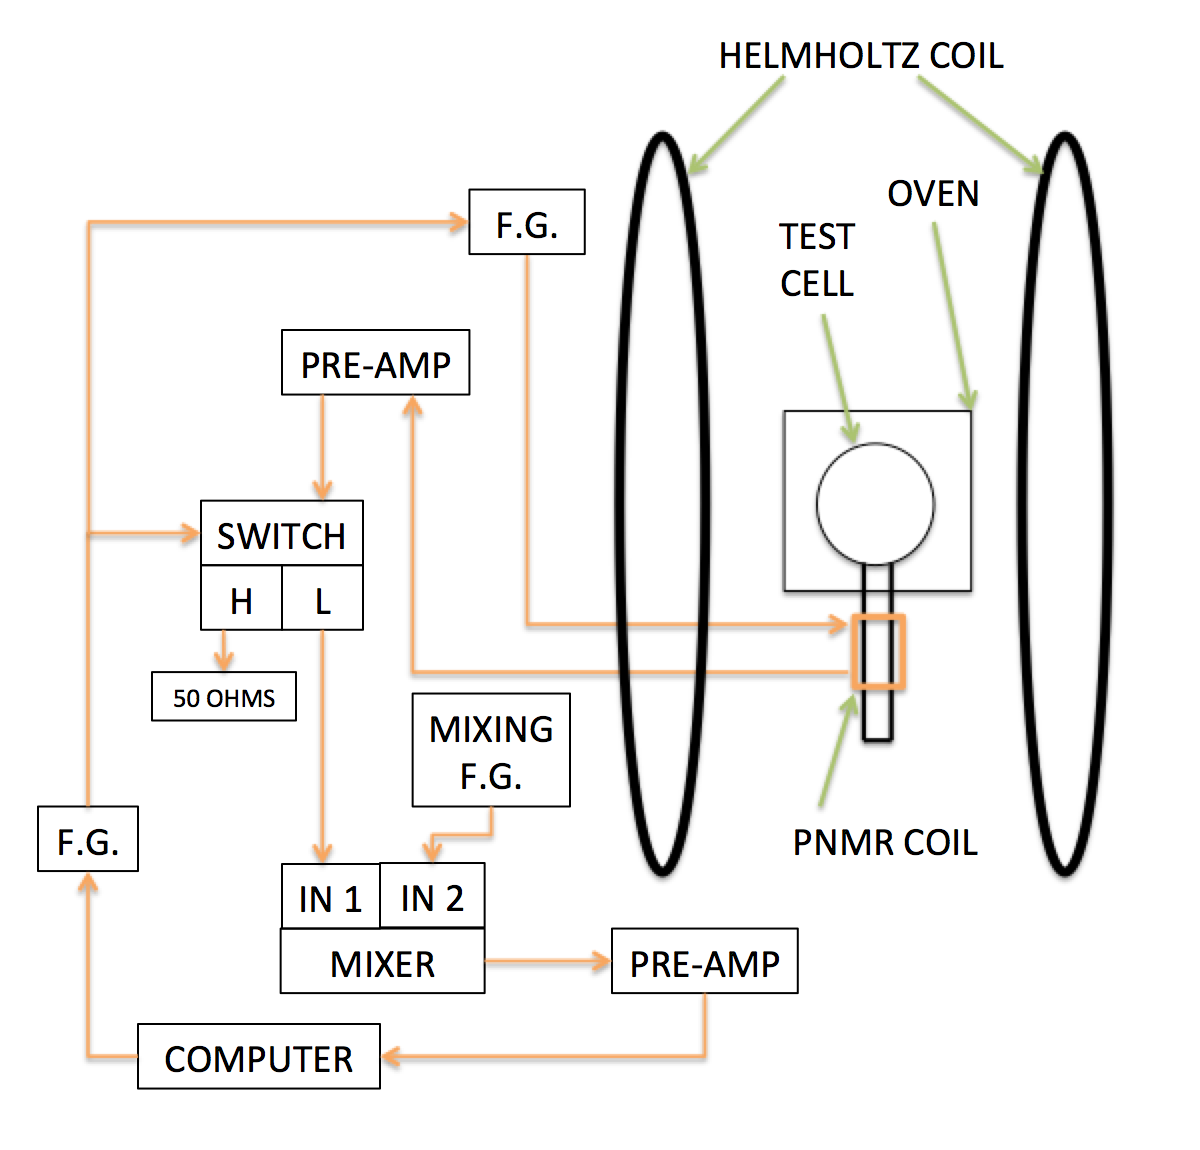
\includegraphics{PNMR_setup.png}}
	\caption{{\bf PNMR setup.}}
	\label{PNMR_setup}
\end{figure}

\emph{et al.}\%
5P$_{\frac{3}{2}}\rightarrow$

\addcontentsline{toc}{chapter}{Bibliography}
\bibliography{ref}

\end{document}